\section{Événements utilisés}\label{chapter-ML-section-evt_gen}
\subsection{Sélection des événements}
about the same as in the analysis (\pT\ cuts, \DEEPTAU, ...)

+ \ele\ele\ and \mu\mu\ channels as well!

\subsection{Génération avec \FASTSIM}

Give the settings used.

Also cite the followings:

\fullcite{FastSim_2011}

\fullcite{FastSim_2014}

\fullcite{FastSim_2017_1}

\fullcite{FastSim_2017_2}

from 50 to 800 GeV

justify by showing plots when trained on smaller mass ranges

below the selections drops everything (plot below)

above problem not solved yet

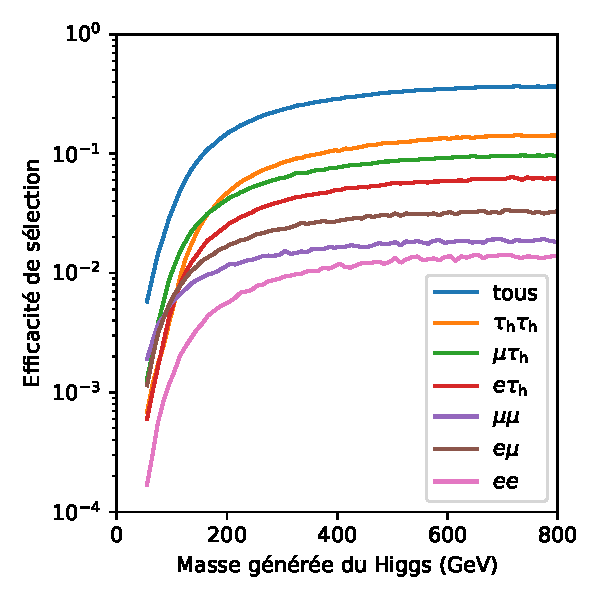
\includegraphics[width=.45\textwidth]{\PhDthesisdir/plots_and_images/my_plots/ML/from_ML_plots/FastSim_NanoAOD_to_NN/ALL_PU2017/plots_Htt_merged_NanoAODSIM_ALL_PU2017-DeepTau_1000/analysis_cuts_efficiency.pdf}

amount of events: 60/20/10 k due to the cut efficiencies 

mass distribution obtained

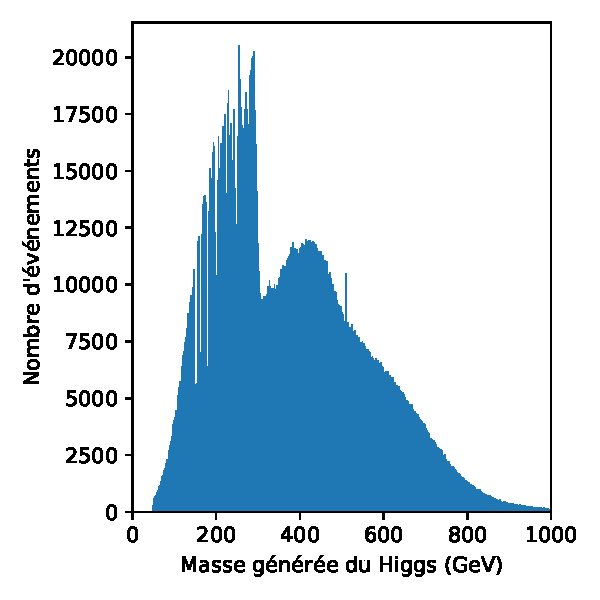
\includegraphics[width=.45\textwidth]{\PhDthesisdir/plots_and_images/my_plots/ML/from_ML_plots/FastSim_NanoAOD_to_NN/ALL_PU2017/plots_Htt_merged_NanoAODSIM_ALL_PU2017-DeepTau/distribution-inclusive-Higgs_mass_gen-raw-all_events.pdf}

weights per steps of 2 GeV

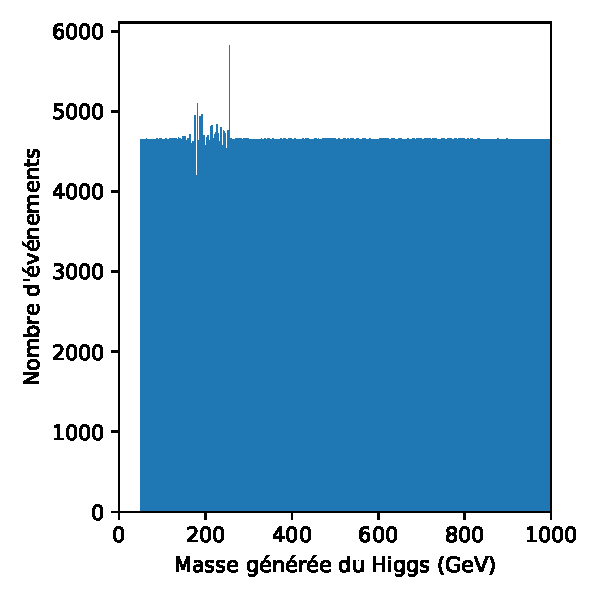
\includegraphics[width=.45\textwidth]{\PhDthesisdir/plots_and_images/my_plots/ML/from_ML_plots/FastSim_NanoAOD_to_NN/ALL_PU2017/plots_Htt_merged_NanoAODSIM_ALL_PU2017-DeepTau/distribution-inclusive-Higgs_mass_gen-weighted-is_train.pdf}

70/20/10 \% fraction for train/valid/test
